%!TEX root = ../main.tex
%
%
\begin{figure}[t!]
\centering
\footnotesize
\begin{tabular}{@{}c@{\;}c@{\;}}
%
%=====================
%
%\rotatebox{90}{\quad\quad Multi-jitter} & 
\begin{tikzpicture}
  \node[anchor=south west,inner sep=0] (image) at (0,0)
  {
    \pdfliteral{ 1 w}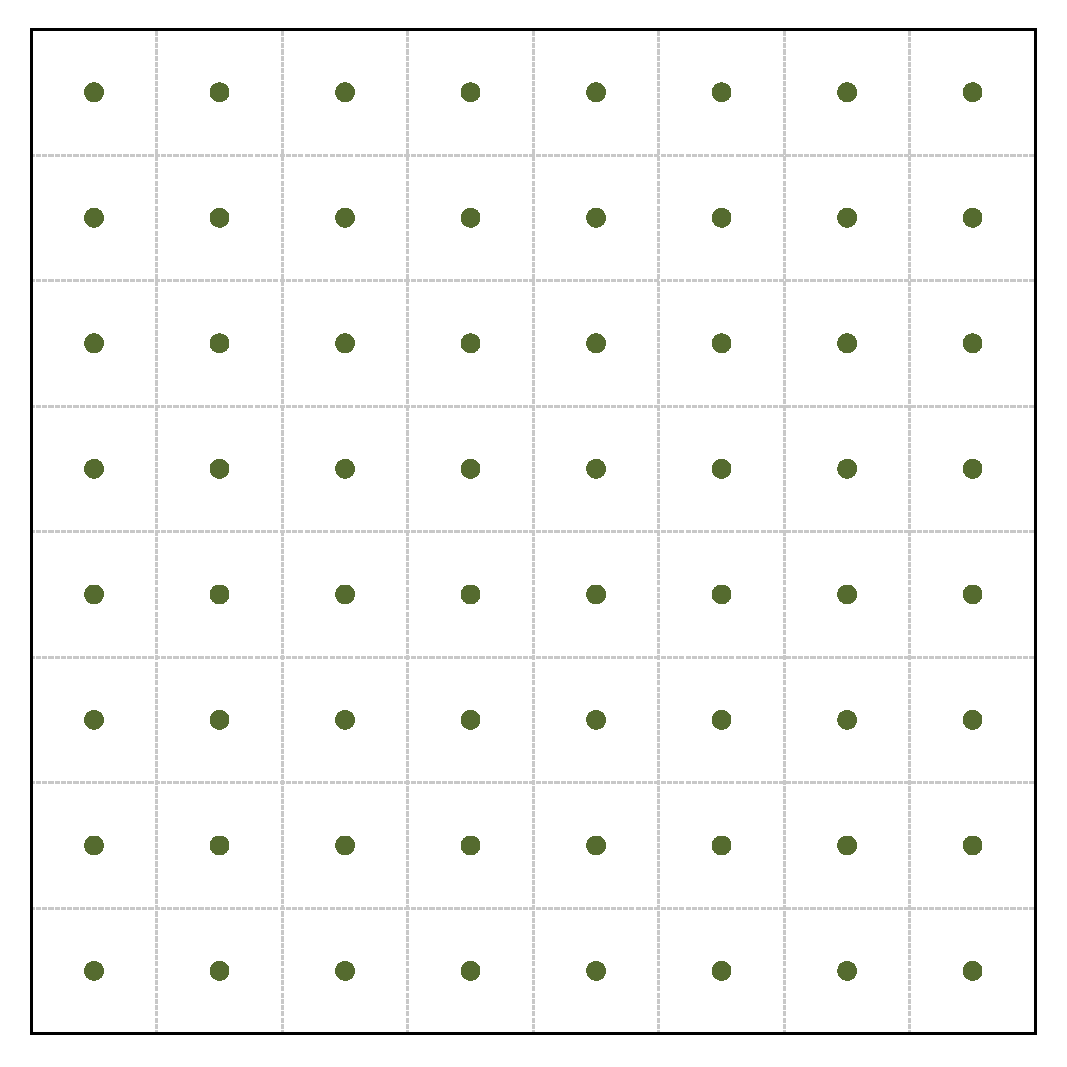
\includegraphics[width=0.4\columnwidth,page=1]{pointset-gridvisualize/points-regular-n64.pdf}
  };
\end{tikzpicture} 
&
\begin{tikzpicture}
  \node[anchor=south west,inner sep=0] (image) at (0,0)
  {
    \pdfliteral{ 1 w}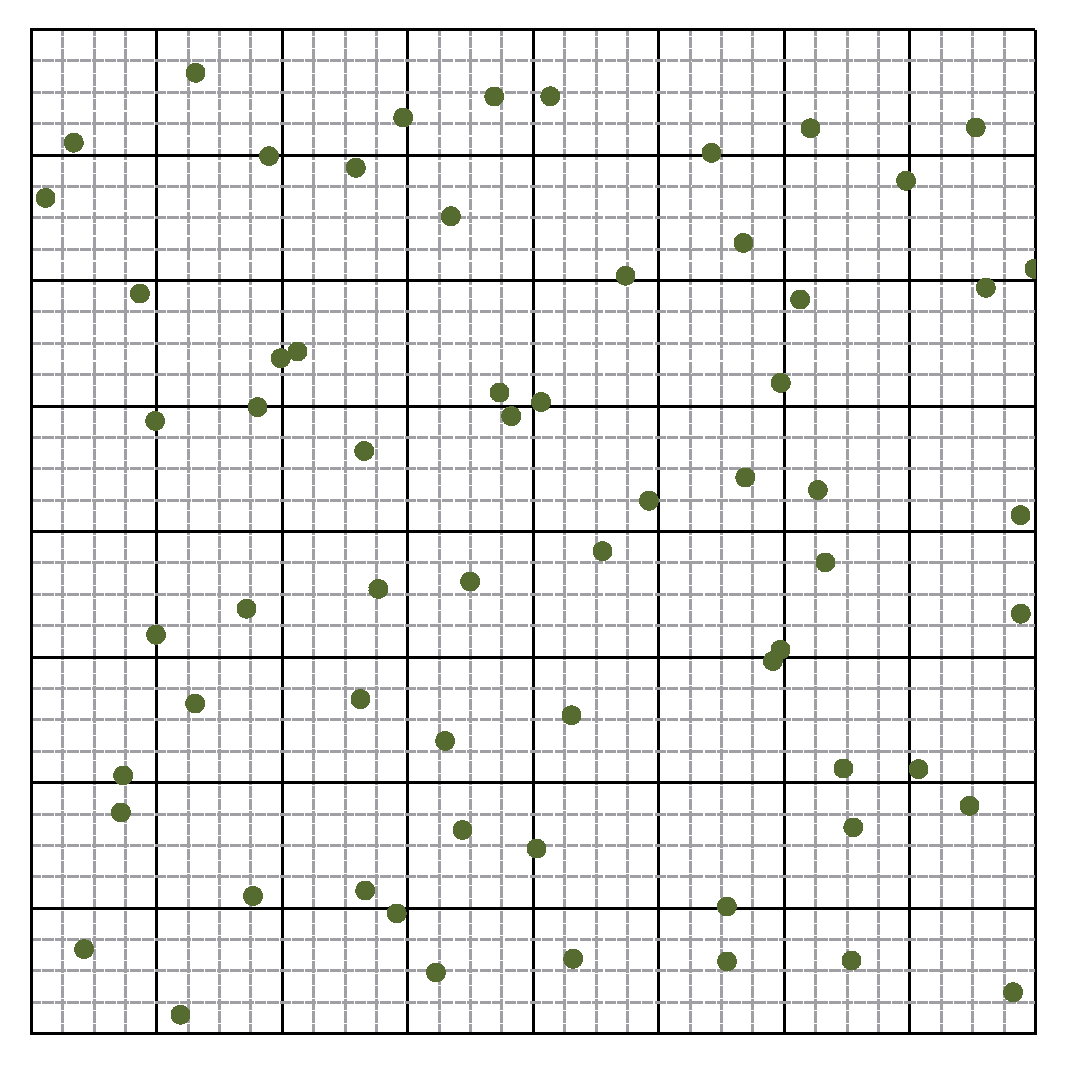
\includegraphics[width=0.4\columnwidth,page=1]{pointset-gridvisualize/points-jitter-n64.pdf}
  };
\end{tikzpicture} 
\\
Regular & Jitter
\\
\begin{tikzpicture}
  \node[anchor=south west,inner sep=0] (image) at (0,0)
  {
    \pdfliteral{ 1 w}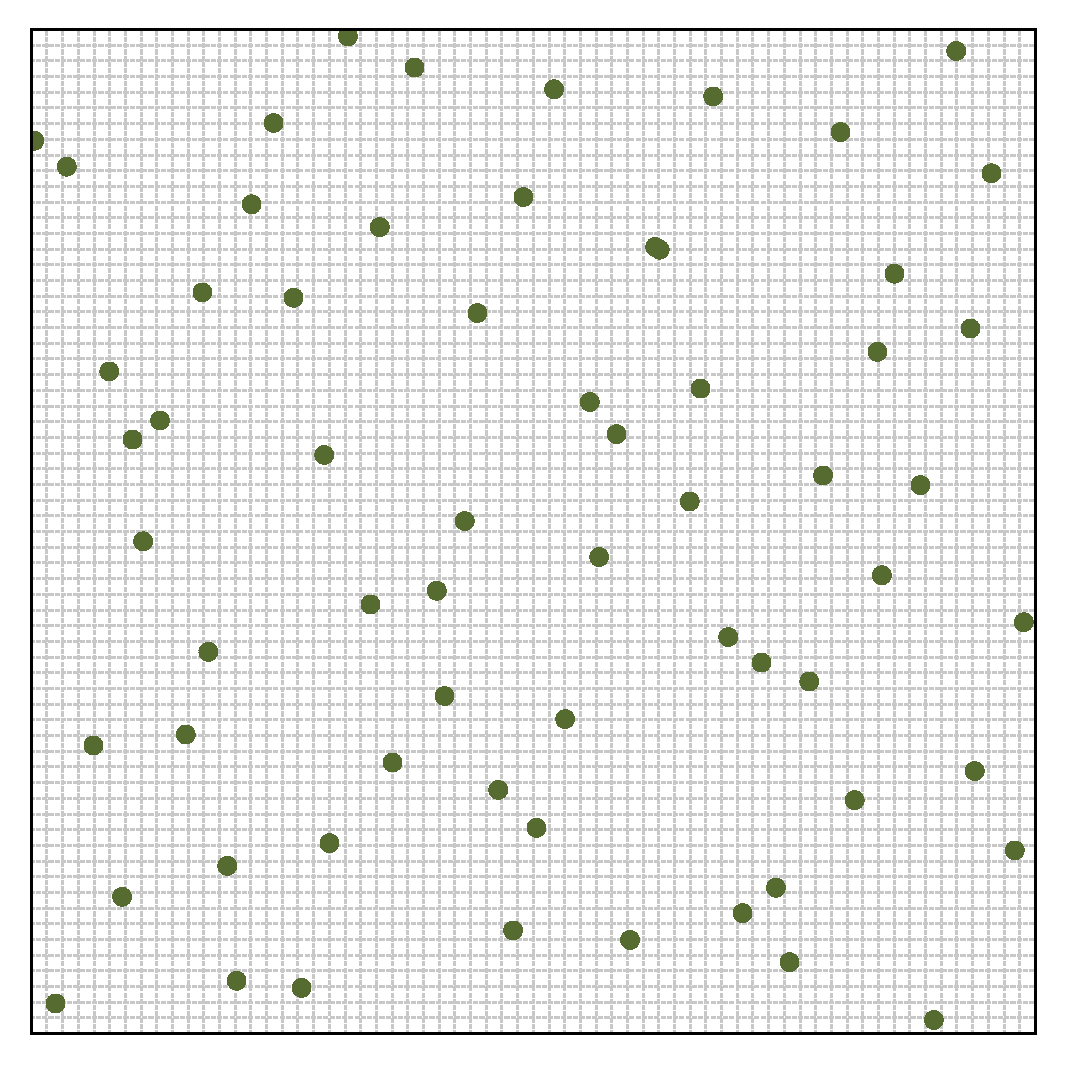
\includegraphics[width=0.4\columnwidth,page=1]{pointset-gridvisualize/points-multijitter-n64.pdf}
  };
\end{tikzpicture} 
&
\begin{tikzpicture}
  \node[anchor=south west,inner sep=0] (image) at (0,0)
  {
    \pdfliteral{ 1 w}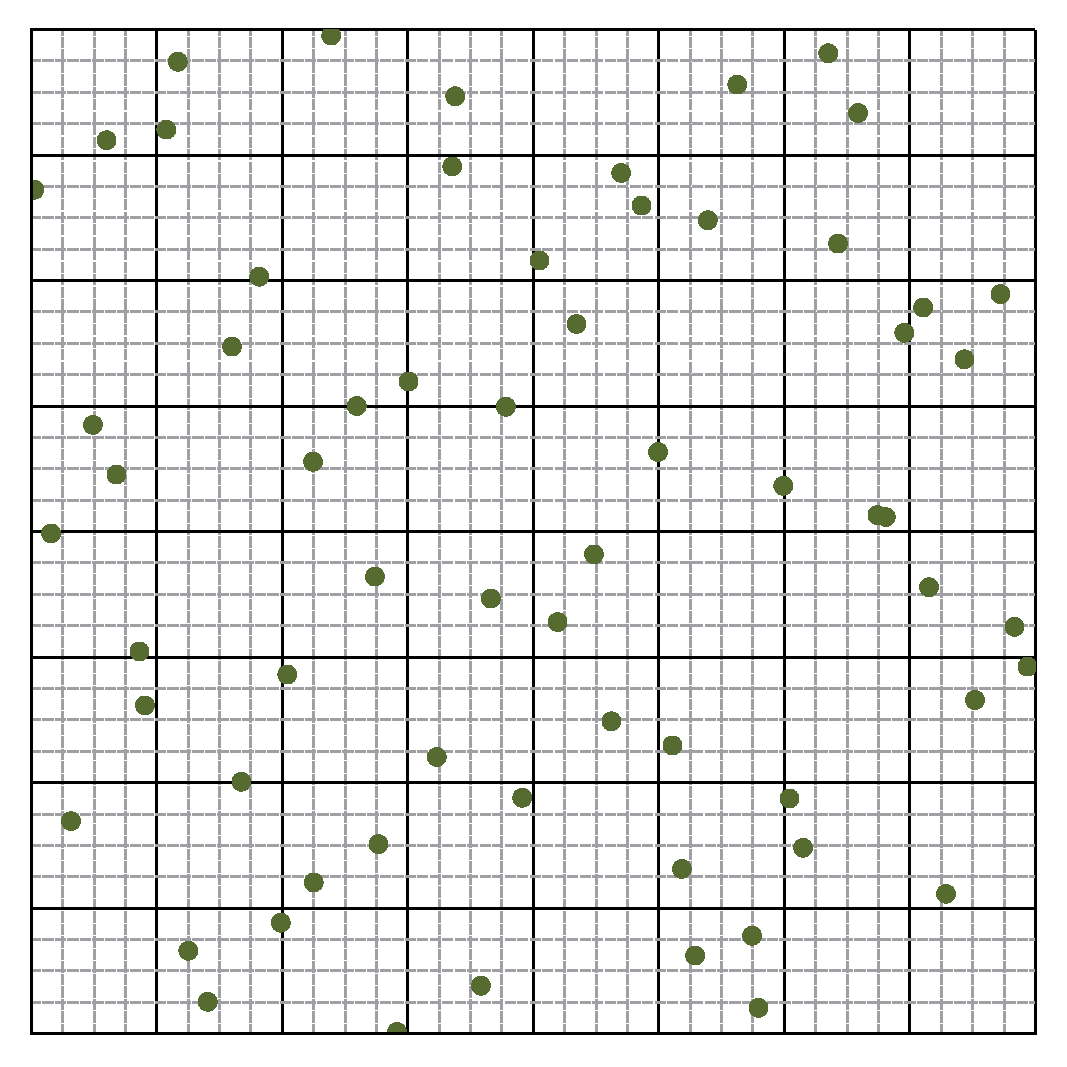
\includegraphics[width=0.4\columnwidth,page=1]{pointset-gridvisualize/points-nrooks-n64.pdf}
  };
\end{tikzpicture}
\\
Multi-Jitter & n-Rooks
\\
\begin{tikzpicture}
  \node[anchor=south west,inner sep=0] (image) at (0,0)
  {
    \pdfliteral{ 1 w}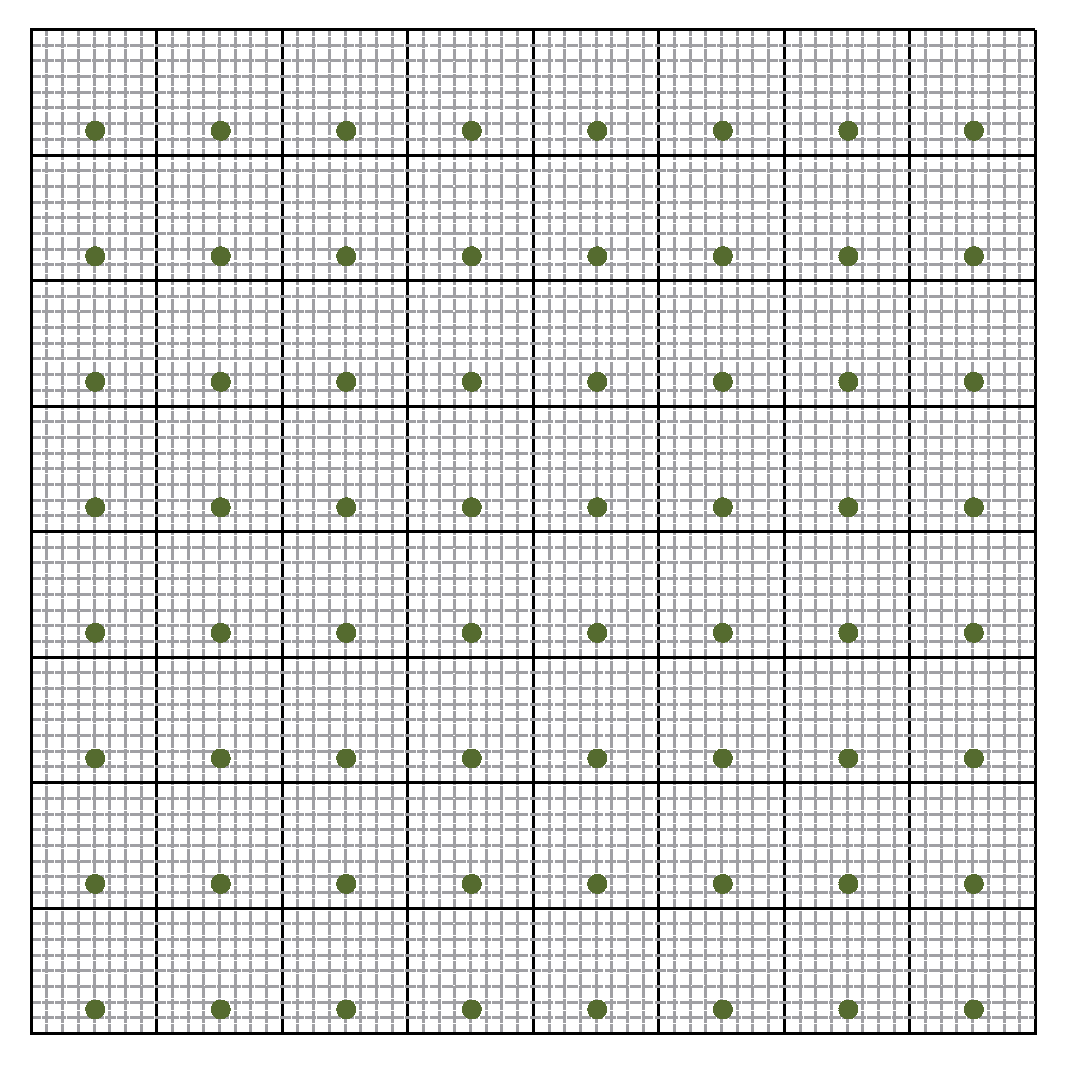
\includegraphics[width=0.4\columnwidth,page=1]{pointset-gridvisualize/points-uniformjitter-n64-1.pdf}
  };
\end{tikzpicture} 
&
\begin{tikzpicture}
  \node[anchor=south west,inner sep=0] (image) at (0,0)
  {
    \pdfliteral{ 1 w}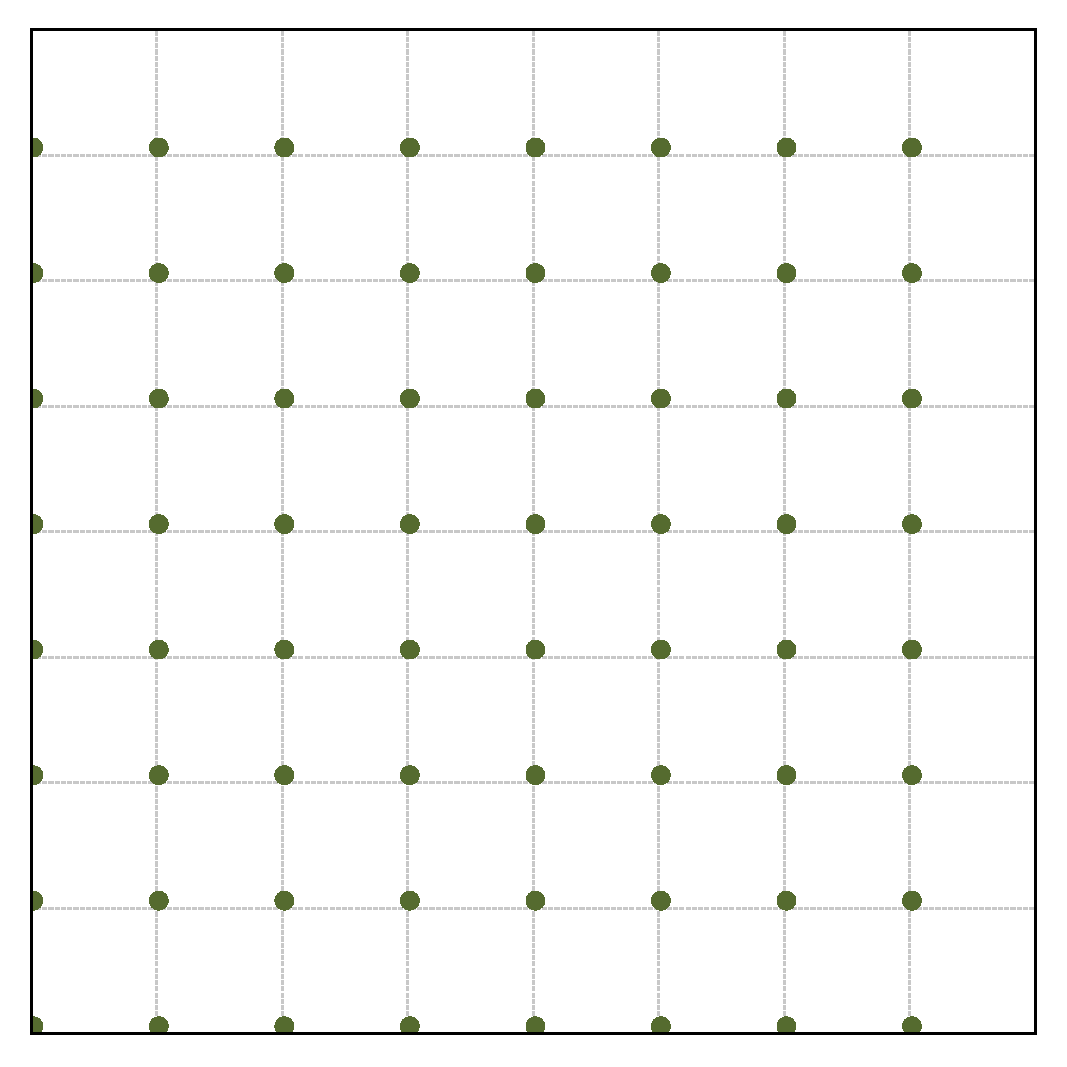
\includegraphics[width=0.4\columnwidth,page=1]{pointset-gridvisualize/points-uniformjitter-n64.pdf}
  };
\end{tikzpicture}
\\
Uniformjitter & Uniformjitter
\\
\end{tabular}
%
\caption{\label{fig:points-grid-visualization}%
Illustration of some sampling patterns.}
\end{figure}